\chapter{Informe de pruebas}
\label{appendix:pruebas}

En el presente anexo se incluyen las pruebas realizadas en el sistema. En el subsistema servidor, nombrado como \textbf{DMPTool - Server}, es donde se centraliza todo el control de la aplicaci�n, los objetos de dominio y las capas de persistencia y comunicaciones, por lo que se han realizado \textit{test cases} para todas y cada una de las capas de dicho sistema, con el fin de asegurar su correcto funcionamiento y obtener los resultados esperados.

Cabe destacar que se han realizado pruebas unitarias (funcionamiento de las clases), pruebas de integraci�n (interacci�n
entre objetos), pruebas de sistema (comunicaci�n entre subsistemas) y pruebas de aceptaci�n
(casos de uso o funcionalidades del sistema), bas�ndose en una combinaci�n de los enfoques de
caja negra y caja blanca, tratando de maximizar la cobertura de instrucciones, considerando m�s de un 80\% de cobertura como aceptable.

Por otra parte, las pruebas realizadas al subsistema cliente, nombrado como \textbf{DMPTool - Client} se refieren a los diferentes \textit{checklist} que se han creado para asegurar el correcto funcionamiento de la interfaz gr�fica, obteniendo el resultado esperado en cada situaci�n, as� como las pruebas para la generaci�n de gr�ficos estad�sticos, mostradas en el Cap�tulo 5.
Como el sistema cliente obtiene todos los datos realizando peticiones al servidor, si se asegura el correcto funcionamiento de este �ltimo, se podr� esperar que los datos recibidos por el cliente sean los correctos. Es por ello que resulta m�s relevante y crucial probar el subsistema servidor.

En las posteriores secciones se presenta el informe obtenido al ejecutar la \textit{suite} de pruebas completas con JUnit en el subsistema servidor, as� como el informe de cobertura obtenido en dicho sistema con Eclemma.

\section{Informe de JUnit}

Una vez dise�ados e implementados los diferentes casos de prueba que integran la \textit{suite} de pruebas para el subsistema servidor, dicha \textit{suite} se ejecuta con \textbf{JUnit} para obtener el resultado de las pruebas. Adem�s, para poder obtener dichos resultados en forma de informe HTML, se ejecut� un tarea de \textit{Ant}, generando el informe de pruebas mostrado en la Figura \ref{fig:JUnit}.

\setlength\fboxsep{0pt}
\setlength\fboxrule{0.5pt}

 \begin{figure}[!htbp]
 \begin{center}
 \fbox{
  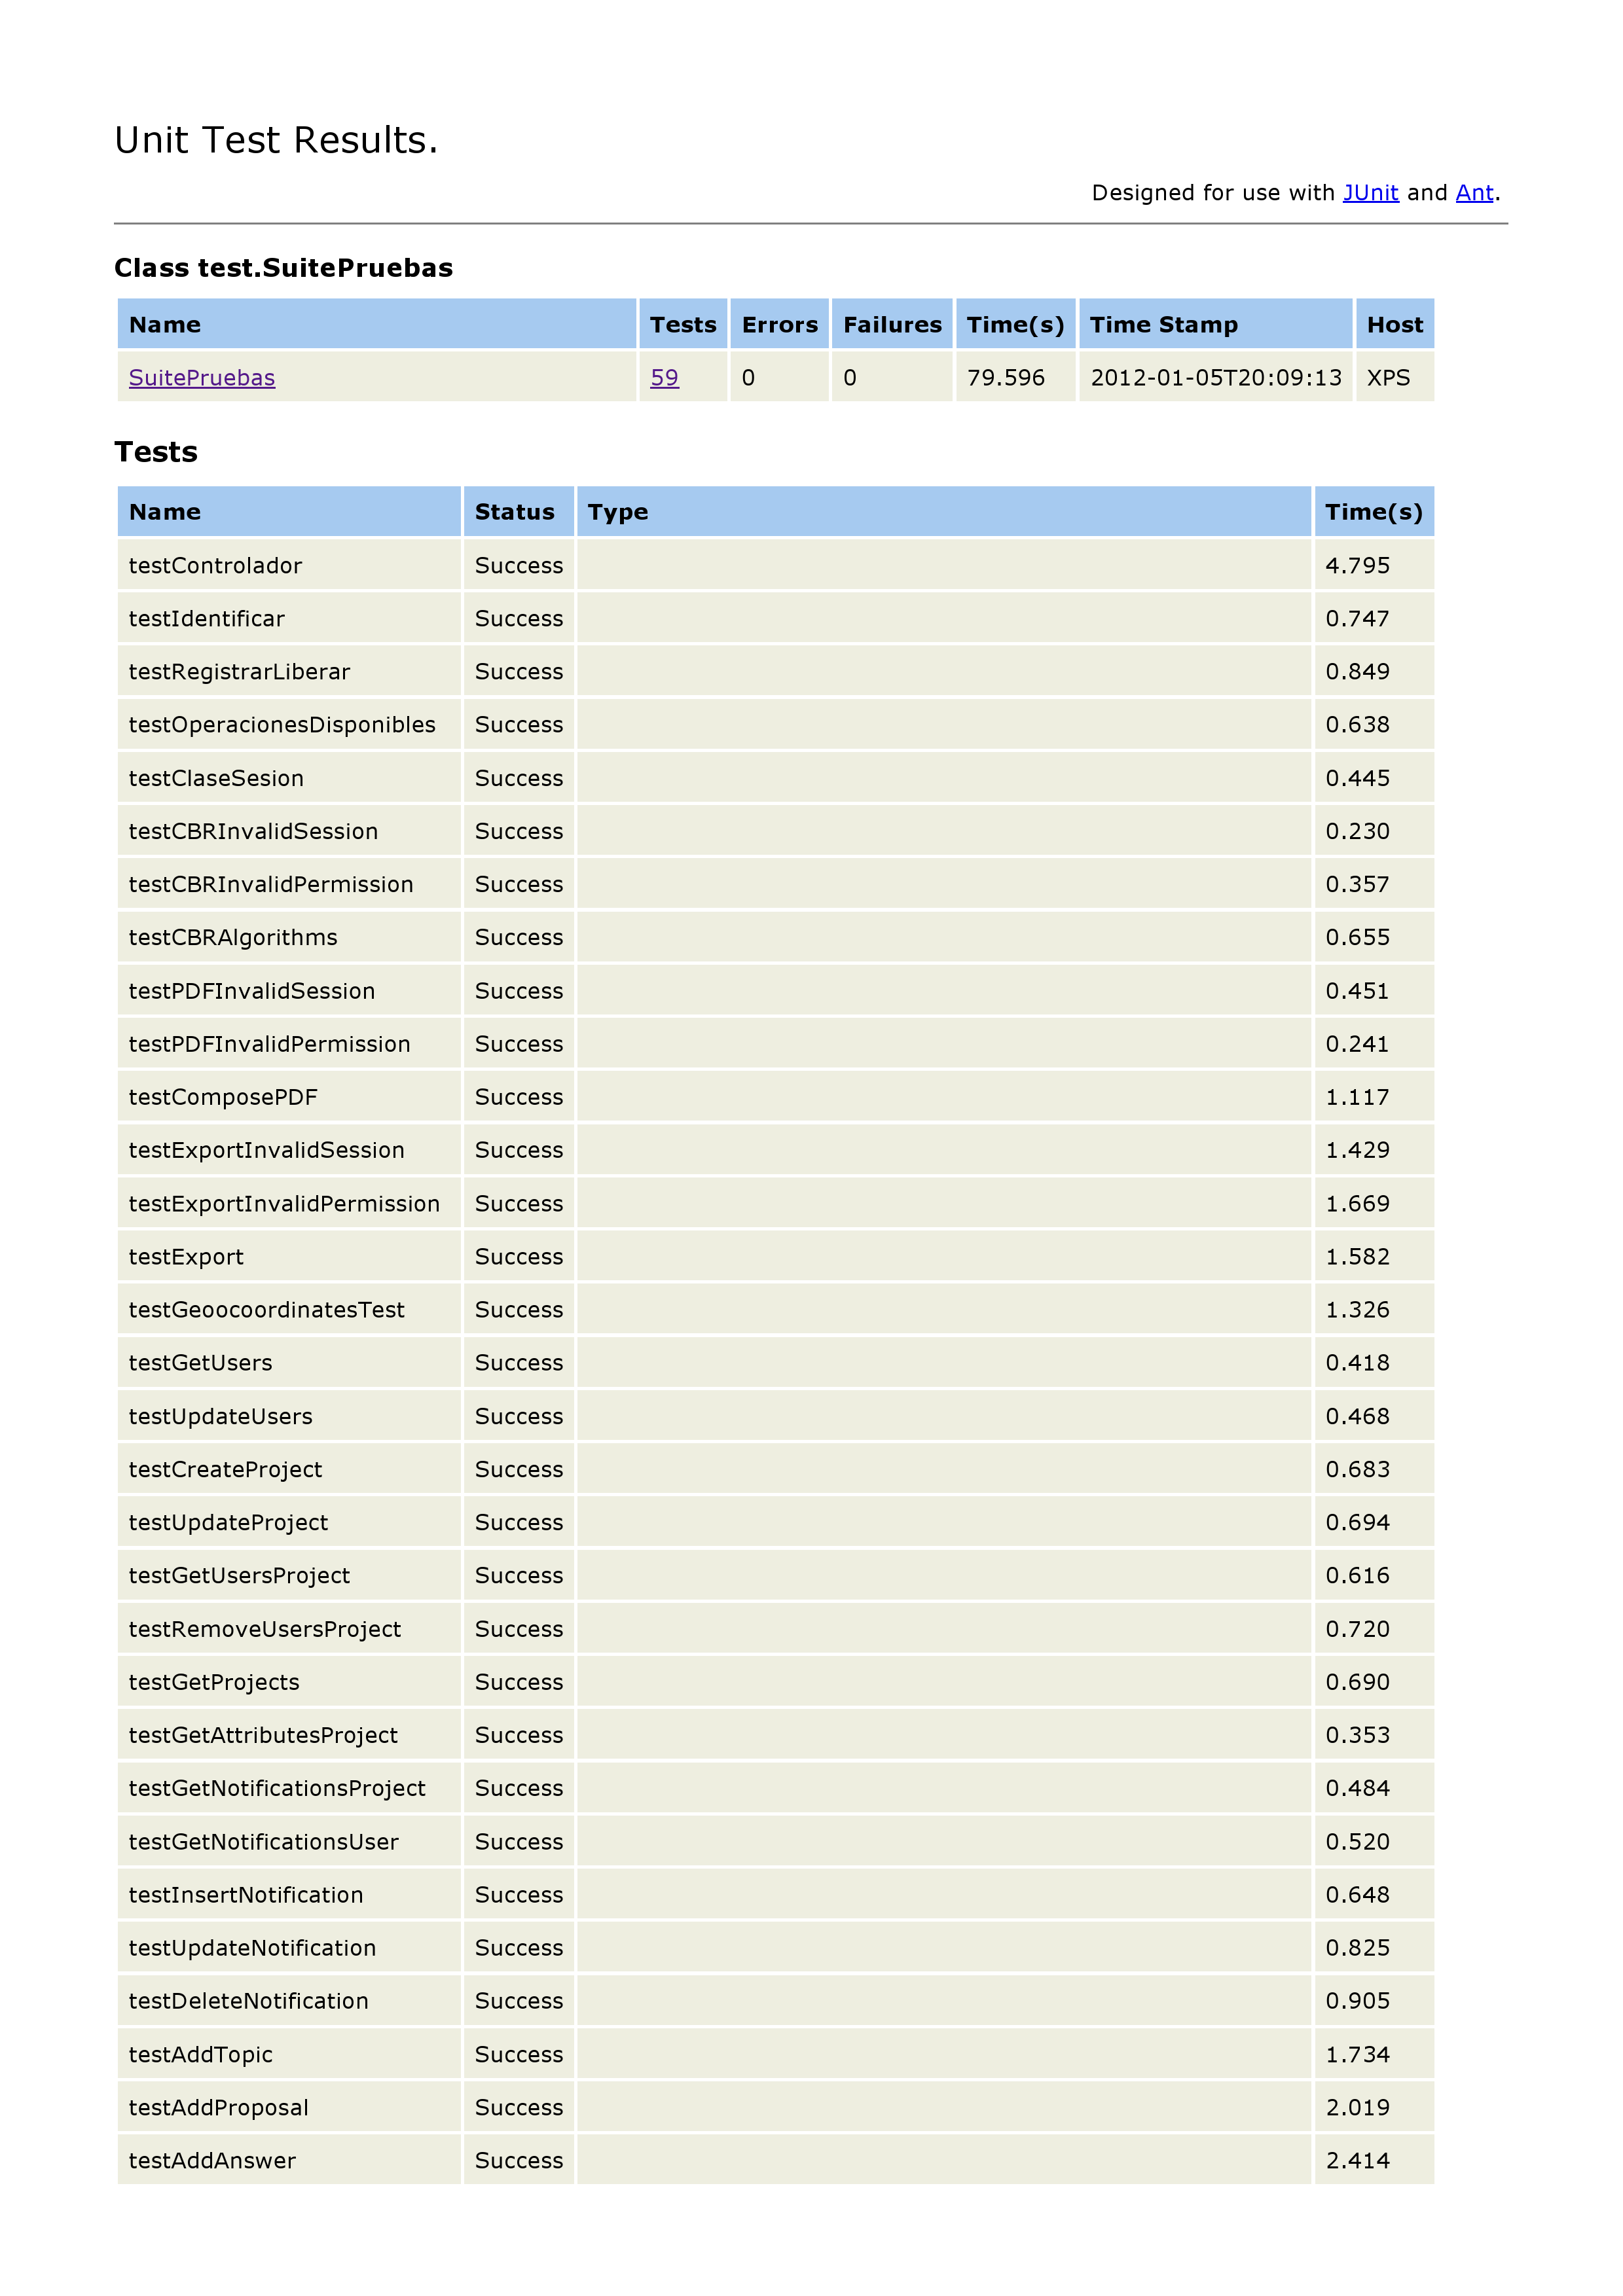
\includegraphics[width=\textwidth, height=\textheight]{Apendices/Pruebas//UnitTest1}}
 \caption*{}
 \label{}
 \end{center}
\end{figure}

\setlength\fboxsep{0pt}
\setlength\fboxrule{0.5pt}
 \begin{figure}[!htbp]
 \begin{center}
 \fbox{
  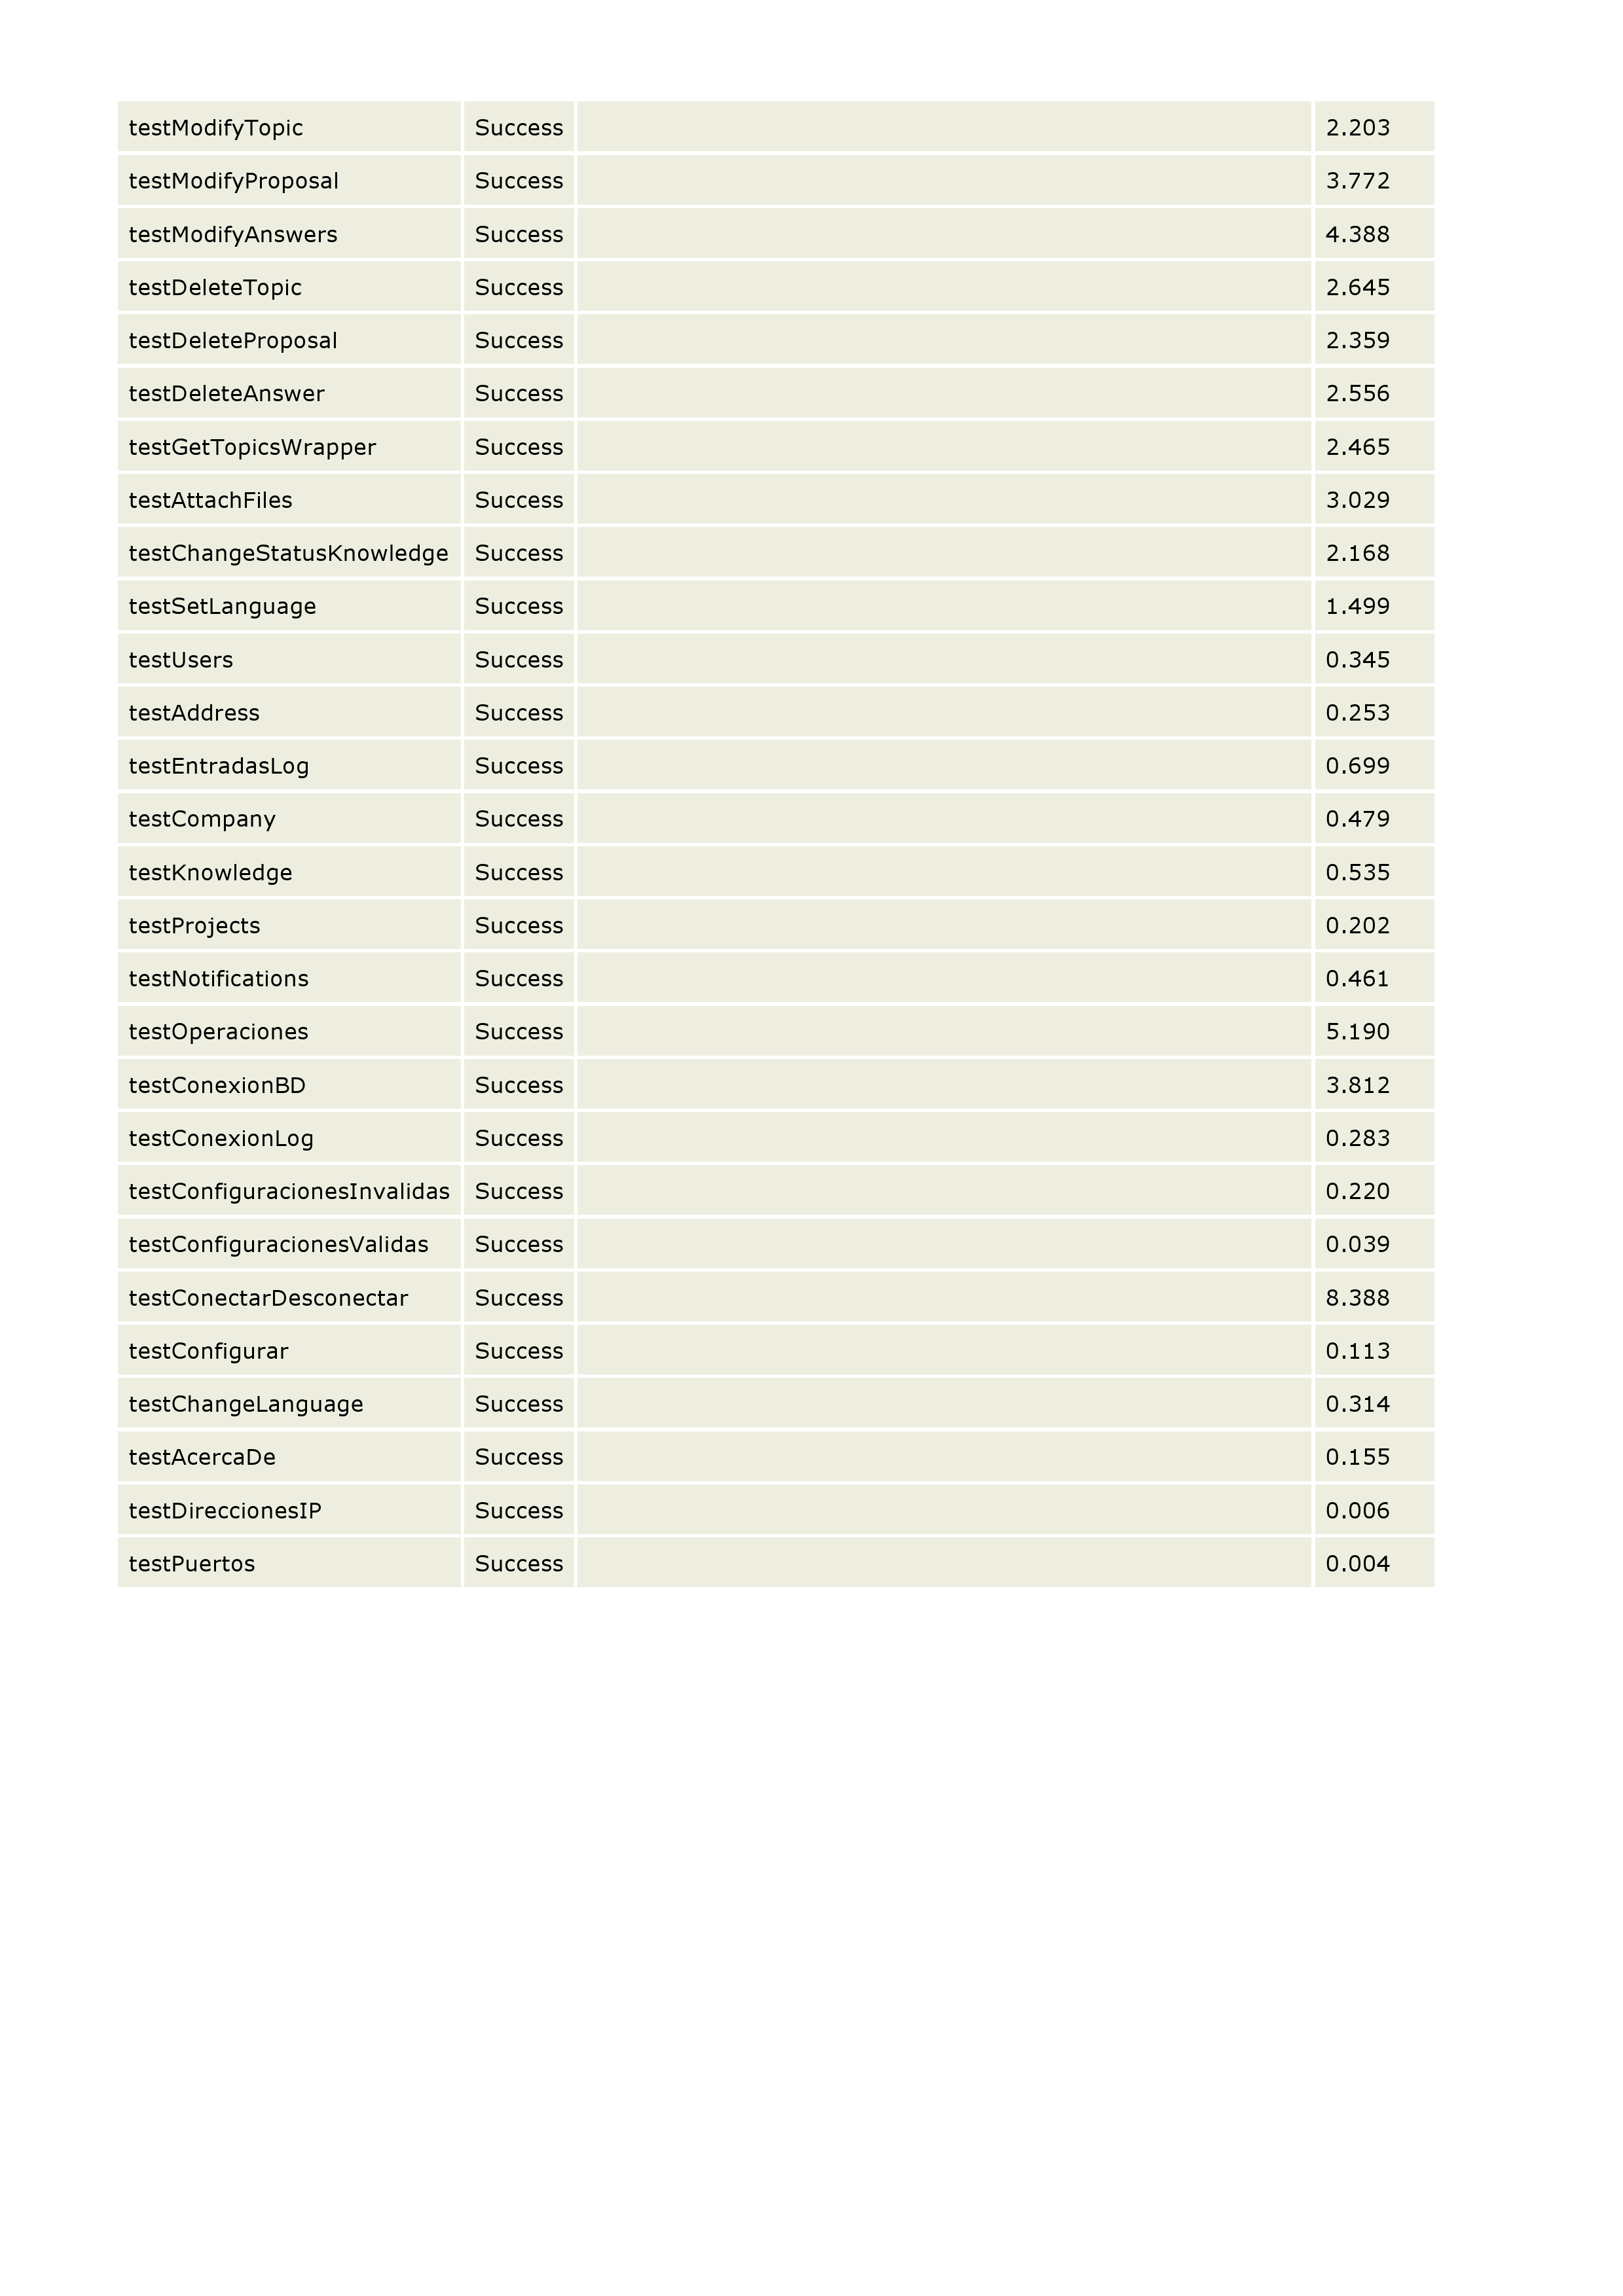
\includegraphics[width=\textwidth, height=\textheight]{Apendices/Pruebas//UnitTest2}}
 \caption{Informe de pruebas de JUnit}
 \label{fig:JUnit}
 \end{center}
\end{figure}

Como se puede apreciar, se dise�aron y ejecutaron 59 casos de prueba para probar todas las capas y clases del sistema servidor, asegurando un funcionamiento correcto de este sistema, que es el que centraliza toda la l�gica de dominio y control.

\section{Informe de cobertura}

Tras ejecutar los casos de prueba para el servidor, y despu�s de corregir los errores que dichas pruebas reflejaron, la \textit{suite} de pruebas dise�ada se ejecuta nuevamente con la herramienta \textbf{Eclemma}, para generar un informe de cobertura de c�digo y comprobar que se ha probado la pr�ctica totalidad de instrucciones.

En la Figura \ref{fig:coberturaTotal} se aprecia el resultado de cobertura obtenido en el sistema servidor que es de un 84\%. Dicha cobertura se desglosa seg�n los paquetes de las diferentes capas que conforman el sistema, cuyos resultados se muestran en la Figura \ref{fig:coberturaPaquetes}.

Como se puede apreciar, existen clases en las que no se alcanza ese umbral de 80\%, debido a que existen ciertos bloques correspondientes al tratamiento
de excepciones que no se han forzado en las pruebas. Dichas excepciones estar�an relacionadas con
problemas de integridad e inconsistencias en las bases de datos, no pudi�ndose dar en �stas, debido
a que el sistema obliga a una correcta inserci�n de datos. De todos modos, si por causas externas
al sistema (por ejemplo, corrupci�n f�sica de los datos) se diesen dichas excepciones, el sistema las
tratar� y notificar� debidamente. 

Para terminar, cabe destacar la capa de control de la l�gica de dominio del sistema, donde se alcanza una cobertura superior al 95\% en la pr�ctica totalidad de sus clases, a excepci�n de la clase \textit{Server}, como se muestra en la Figura \ref{fig:coberturaControl}. Dicha clase se corresponde con el patr�n \textbf{Fachada} del sistema servidor y disminuye la cobertura porque algunos de sus bloques corresponden al control de excepciones que no se han podido forzar en las pruebas, como se ha comentado anteriormente.

\setlength\fboxsep{0pt}
\setlength\fboxrule{0.5pt}
 \begin{figure}[!htbp]
 \begin{center}
 \fbox{
  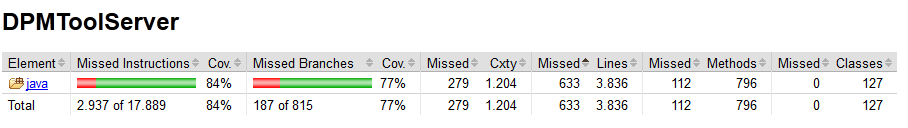
\includegraphics[width=\textwidth]{Apendices/Pruebas//coberturaTotal}}
 \caption{Informe de cobertura para el sistema servidor}
 \label{fig:coberturaTotal}
 \end{center}
\end{figure}

\setlength\fboxsep{0pt}
\setlength\fboxrule{0.5pt}
 \begin{figure}[!htbp]
 \begin{center}
 \fbox{
  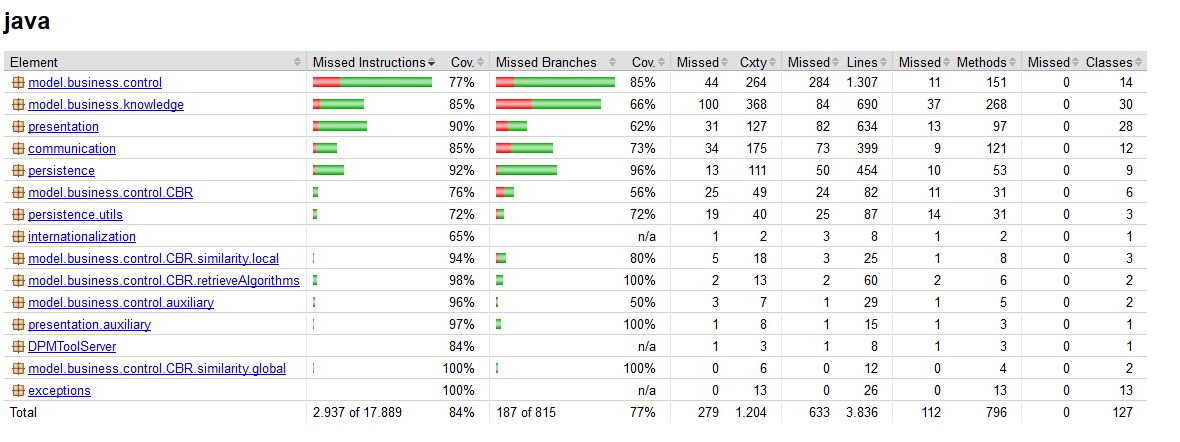
\includegraphics[width=\textwidth]{Apendices/Pruebas//coberturaPaquetes}}
 \caption{Informe de cobertura para las diferentes capas del sistema servidor}
 \label{fig:coberturaPaquetes}
 \end{center}
\end{figure}

\setlength\fboxsep{0pt}
\setlength\fboxrule{0.5pt}
 \begin{figure}[!htbp]
 \begin{center}
 \fbox{
  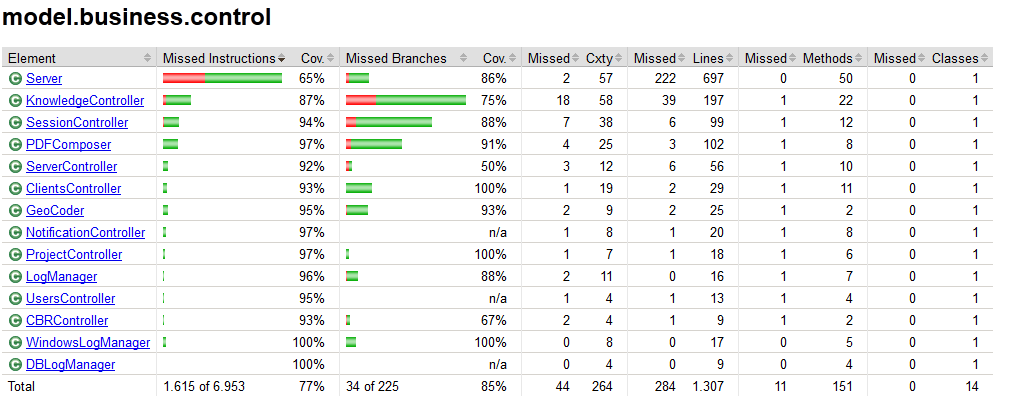
\includegraphics[width=\textwidth]{Apendices/Pruebas//coberturaControl}}
 \caption{Informe de cobertura para la capa de control de la l�gica de dominio del sistema servidor}
 \label{fig:coberturaControl}
 \end{center}
\end{figure}